\section*{Question 2:}
Exercise 8.4: 

For two queries in the CACM collection, generate two uninterpolated recall precision graphs, a table of interpolated precision values at standard recall levels, and the average interpolated recall-precision graph.

\subsection*{Answer:}

I decided to run query \#13 "code optimization for space efficiency" and query \#27 ``memory management aspects of perating systems''.

I created the file named ``84.json'' and saved the queries in it as directed by Galago ``batch-search'' command help.

\lstinputlisting[language=XML, breakatwhitespace=〈false), label=The content of 84.json, caption= The content of 84.json]{Q2/84.json}

I generated the ranking list using Galago from the command line:

\begin{lstlisting}[breakatwhitespace=〈false)]
hussam@hussam-HP-Compaq-nc8430-GE542UP-ABA:~/Desktop/galago/galago-bin/bin$ ./galago batch-search --index=./index --requested=10 84.json
CACM-13 Q0 /home/hussam/Desktop/galago/galago-bin/bin/cacm/CACM-2897.html 1 -6.20214617 galago
CACM-13 Q0 /home/hussam/Desktop/galago/galago-bin/bin/cacm/CACM-2033.html 2 -6.28636814 galago
CACM-13 Q0 /home/hussam/Desktop/galago/galago-bin/bin/cacm/CACM-1947.html 3 -6.36386467 galago
CACM-13 Q0 /home/hussam/Desktop/galago/galago-bin/bin/cacm/CACM-2559.html 4 -6.45008887 galago
CACM-13 Q0 /home/hussam/Desktop/galago/galago-bin/bin/cacm/CACM-2491.html 5 -6.45483869 galago
CACM-13 Q0 /home/hussam/Desktop/galago/galago-bin/bin/cacm/CACM-2680.html 6 -6.52951010 galago
CACM-13 Q0 /home/hussam/Desktop/galago/galago-bin/bin/cacm/CACM-2701.html 7 -6.54338217 galago
CACM-13 Q0 /home/hussam/Desktop/galago/galago-bin/bin/cacm/CACM-1886.html 8 -6.54934530 galago
CACM-13 Q0 /home/hussam/Desktop/galago/galago-bin/bin/cacm/CACM-2944.html 9 -6.56475305 galago
CACM-13 Q0 /home/hussam/Desktop/galago/galago-bin/bin/cacm/CACM-2537.html 10 -6.58501681 galago
CACM-27 Q0 /home/hussam/Desktop/galago/galago-bin/bin/cacm/CACM-2297.html 1 -5.78832924 galago
CACM-27 Q0 /home/hussam/Desktop/galago/galago-bin/bin/cacm/CACM-1752.html 2 -5.98368977 galago
CACM-27 Q0 /home/hussam/Desktop/galago/galago-bin/bin/cacm/CACM-2902.html 3 -6.02077716 galago
CACM-27 Q0 /home/hussam/Desktop/galago/galago-bin/bin/cacm/CACM-2319.html 4 -6.04039597 galago
CACM-27 Q0 /home/hussam/Desktop/galago/galago-bin/bin/cacm/CACM-2406.html 5 -6.04959217 galago
CACM-27 Q0 /home/hussam/Desktop/galago/galago-bin/bin/cacm/CACM-2740.html 6 -6.07650436 galago
CACM-27 Q0 /home/hussam/Desktop/galago/galago-bin/bin/cacm/CACM-1725.html 7 -6.08352717 galago
CACM-27 Q0 /home/hussam/Desktop/galago/galago-bin/bin/cacm/CACM-2358.html 8 -6.08425902 galago
CACM-27 Q0 /home/hussam/Desktop/galago/galago-bin/bin/cacm/CACM-2988.html 9 -6.10546471 galago
CACM-27 Q0 /home/hussam/Desktop/galago/galago-bin/bin/cacm/CACM-2357.html 10 -6.13047371 galago
\end{lstlisting}

I downloaded the relevance judgment file ``cacm.rel''. The section for query 13 and 27 is:

\begin{lstlisting}[breakatwhitespace=〈false)]
13 Q0 CACM-115 1
13 Q0 CACM-1223 1
13 Q0 CACM-1231 1
13 Q0 CACM-1551 1
13 Q0 CACM-1625 1
13 Q0 CACM-1795 1
13 Q0 CACM-1807 1
13 Q0 CACM-1947 1
13 Q0 CACM-2495 1
13 Q0 CACM-2579 1
13 Q0 CACM-2897 1
27 Q0 CACM-1641 1
27 Q0 CACM-1642 1
27 Q0 CACM-1750 1
27 Q0 CACM-1752 1
27 Q0 CACM-1879 1
27 Q0 CACM-1884 1
27 Q0 CACM-1901 1
27 Q0 CACM-2095 1
27 Q0 CACM-2297 1
27 Q0 CACM-2435 1
27 Q0 CACM-2481 1
27 Q0 CACM-2498 1
27 Q0 CACM-2560 1
27 Q0 CACM-2596 1
27 Q0 CACM-2669 1
27 Q0 CACM-2734 1
27 Q0 CACM-2747 1
27 Q0 CACM-2768 1
27 Q0 CACM-2798 1
27 Q0 CACM-2818 1
27 Q0 CACM-2859 1
27 Q0 CACM-2864 1
27 Q0 CACM-2902 1
27 Q0 CACM-2918 1
27 Q0 CACM-2955 1
27 Q0 CACM-2983 1
27 Q0 CACM-2988 1
27 Q0 CACM-3000 1
27 Q0 CACM-3052 1
\end{lstlisting}

Therefore:

The number of relevant documents in the collection for query \#13 is 11.

The number of relevant documents in the collection for query \#27 is 29.

Each document in the result set can be identified as a ``Hit'' or ``Miss''.

Precision = Number of relevant documents retrieved / number of retrieved documents

\textbf{For query \#13}:

\begin{longtable}{ |p{1cm}|p{4cm}|p{3cm}|p{2cm}|p{2cm}| } 
\hline
Result & File Name & Hit/Miss & Precision & Recall\\
\hline
1 & CACM-2897.html & Hit & 1.0 & 0.5 \\
\hline
2 & CACM-2033.html & Miss & 0.5 & 0.5 \\
\hline
3 & CACM-1947.html & Hit & 0.67 & 1.0 \\
\hline
4 & CACM-2559.html & Miss & 0.5 & 1.0 \\
\hline
5 & CACM-2491.html & Miss & 0.4 & 1.0 \\
\hline
6 & CACM-2680.html & Miss & 0.33 & 1.0 \\
\hline
7 & CACM-2701.html & Miss & 0.29 & 1.0 \\
\hline
8 & CACM-1886.html & Miss & 0.25 & 1.0 \\
\hline
9 & CACM-2944.html & Miss  & 0.22 & 1.0 \\
\hline
10 & CACM-2537.html & Miss & 0.2 & 1.0 \\
\hline
\end{longtable}

It is time to plot uninterpolated Precision vs Recall for query \#13.

The points are saved in the file ``q13.csv''. I used R to create the graph.

\pagebreak

\textbf{Uninterpolated:}

\begin{lstlisting}[breakatwhitespace=〈false)]
q13 <- read.csv("q13.csv", header = TRUE)
plot(q13$Recall, q13$Precision, type = "o", col="red" , xlab = "Recall", ylab = "Precision", main = "Query 13 Precision vs Recall", xlim = c(0,1), ylim = c(0,1))
\end{lstlisting}

\begin{figure}[h]
\caption{Uninterpolated Precision VS Recall for Query 13}
\centering
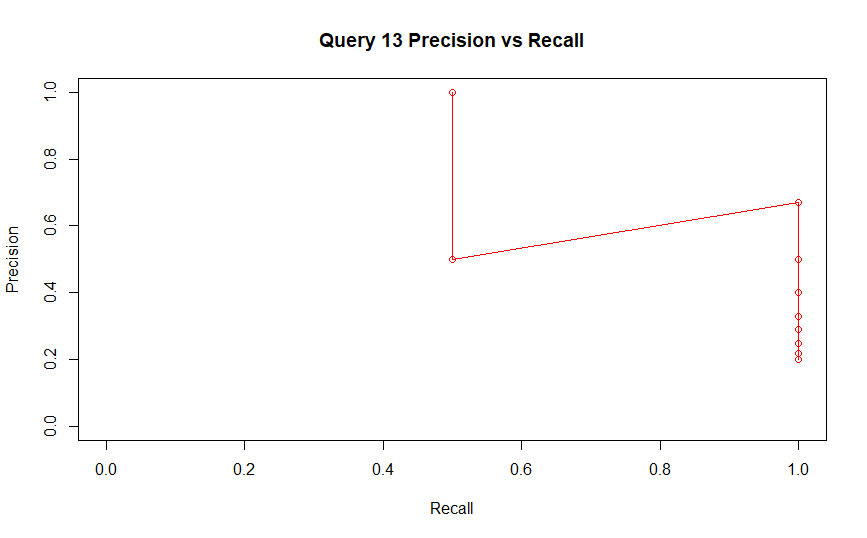
\includegraphics[scale=0.5]{Q2/upvrq13.png}
\end{figure}

\pagebreak

\textbf{For query \#27}:

\begin{longtable}{ |p{1cm}|p{4cm}|p{3cm}|p{2cm}|p{2cm}| } 
\hline
Result & File Name & Hit/Miss & Precision & Recall\\
\hline
1 & CACM-2297.html & Hit & 1.0 & 0.25 \\
\hline
2 & CACM-1752.html & Hit & 1.0 & 0.0.5 \\
\hline
3 & CACM-2902.html & Hit & 1.0 & 0.75 \\
\hline
4 & CACM-2319.html & Miss & 0.75 & 0.75 \\
\hline
5 & CACM-2406.html & Miss & 0.6 & 0.75 \\
\hline
6 & CACM-2740.html & Miss & 0.5 & 0.75 \\
\hline
7 & CACM-1725.html & Miss & 0.43 & 0.75 \\
\hline
8 & CACM-2358.html & Miss & 0.38 & 0.75 \\
\hline
9 & CACM-2988.html & Hit & 0.44 & 1.0 \\
\hline
10 & CACM-2357.html & Miss & 0.4 & 1.0 \\
\hline
\end{longtable}

It is time to plot uninterpolated Precision vs Recall for query \#27.

The points are saved in the file ``q27.csv''. I used R to create the graph.

\textbf{Uninterpolated:}

\begin{lstlisting}[breakatwhitespace=〈false)]
q27 <- read.csv("q27.csv", header = TRUE)
plot(q27$Recall, q27$Precision, type = "o", col="red" , xlab = "Recall", ylab = "Precision", main = "Query 27 Precision vs Recall", xlim = c(0,1), ylim = c(0,1))
\end{lstlisting}


\begin{figure}[h]
\caption{Uninterpolated Precision VS Recall for Query 27}
\centering
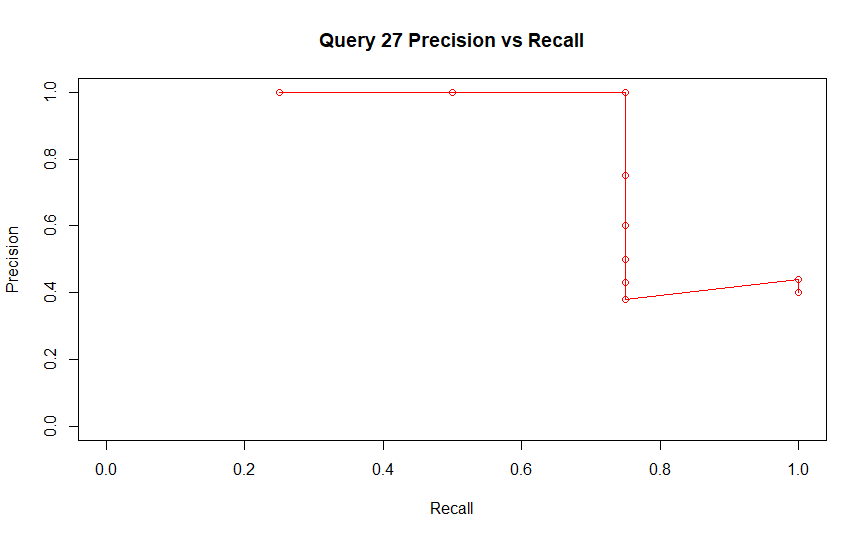
\includegraphics[scale=0.5]{Q2/upvrq27.png}
\end{figure}


\textbf{Interpolated:}
It's time to create a table of interpolated precision values at standard recall levels. By definition, the interpolated precision at any recall level is the maximum precision observed in any recall-precision point at a higher recall level.

\begin{longtable}{|p{1cm}|p{0.7cm}|p{0.7cm}|p{0.7cm}|p{0.7cm}|p{0.7cm}|p{0.7cm}|p{0.7cm}|p{0.7cm}|p{0.7cm}|p{0.7cm}|p{0.7cm}|} 
\hline
Recall & 0.0 & 0.1 & 0.2 & 0.3 & 0.4 & 0.5 & 0.6 & 0.7 & 0.8 & 0.9 & 1.0\\
\hline
Q13 & 1.0 & 1.0 & 1.0 & 1.0 & 1.0 & 1.0 & 0.67 & 0.67 & 0.67 & 0.67 & 0.67\\
\hline
Q27 & 1.0 & 1.0 & 1.0 & 1.0 & 1.0 & 1.0 & 1.0 & 1.0 & 0.75 & 0.44 & 0.44\\
\hline
AVG & 1.0 & 1.0 & 1.0 & 1.0 & 1.0 & 1.0 & 0.84 & 0.84 & 0.71 & 0.56 & 0.56\\
\hline
\end{longtable}

\begin{lstlisting}[breakatwhitespace=〈false)]
q13 <- read.csv("iq13.csv", header = TRUE)
plot(q13$Recall, q13$Precision, type = "o", col="red" , xlab = "Recall", ylab = "Precision", main = "Query 13 interpolated Precision vs Recall", xlim = c(0,1), ylim = c(0,1))
\end{lstlisting}

\begin{figure}[h]
\caption{Interpolated Precision VS Recall for Query 13}
\centering
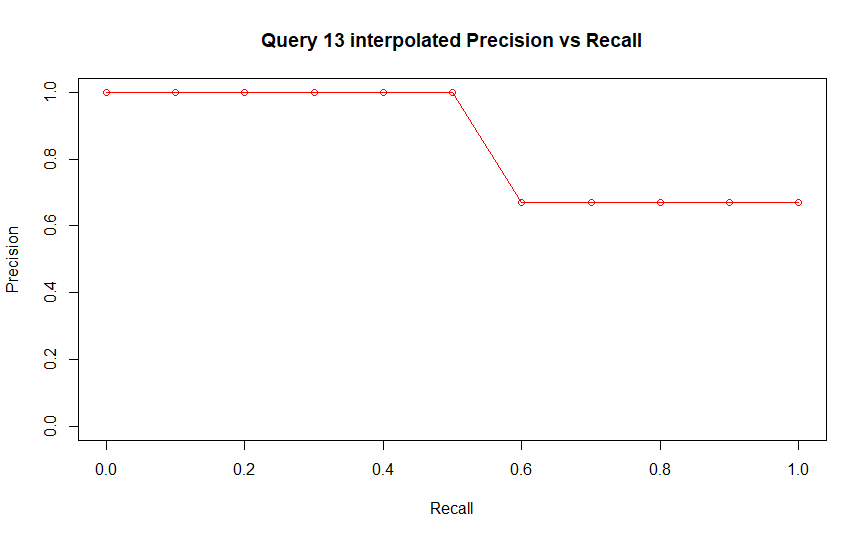
\includegraphics[scale=0.5]{Q2/ipvrq13.png}
\end{figure}


\begin{lstlisting}[breakatwhitespace=〈false)]
q27 <- read.csv("iq27.csv", header = TRUE)
plot(q27$Recall, q27$Precision, type = "o", col="red" , xlab = "Recall", ylab = "Precision", main = "Query 27 interpolated Precision vs Recall", xlim = c(0,1), ylim = c(0,1))
\end{lstlisting}


\begin{figure}[h]
\caption{Interpolated Precision VS Recall for Query 27}
\centering
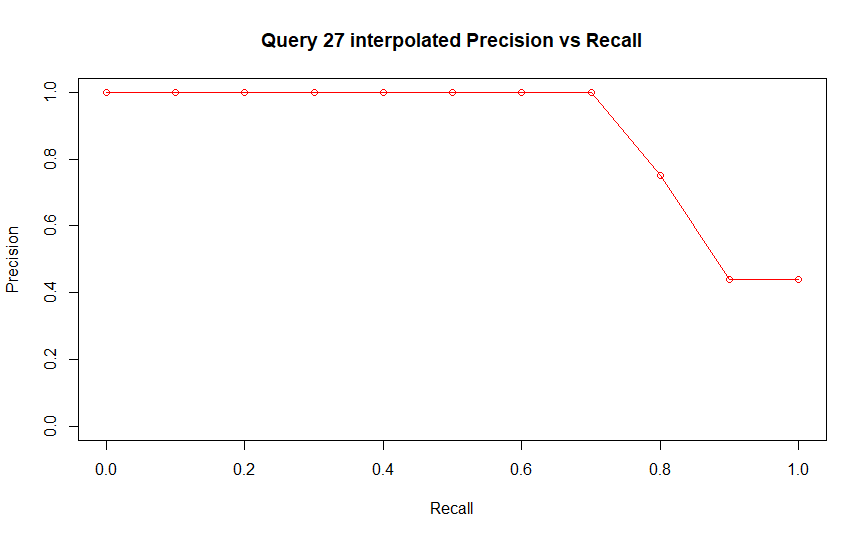
\includegraphics[scale=0.5]{Q2/ipvrq27.png}
\end{figure}

\textbf{The average interpolated recall-precision graph:}

\begin{lstlisting}[breakatwhitespace=〈false)]
a <- read.csv("a.csv", header = TRUE)
plot(a$Recall, a$Precision, type = "o", col="red" , xlab = "Recall", ylab = "Precision", main = "The average interpolated Precision vs Recall for Query 13 and 27", xlim = c(0,1), ylim = c(0,1))
\end{lstlisting}


\begin{figure}[h]
\caption{The average interpolated Precision vs Recall for Query 13 and 27}
\centering
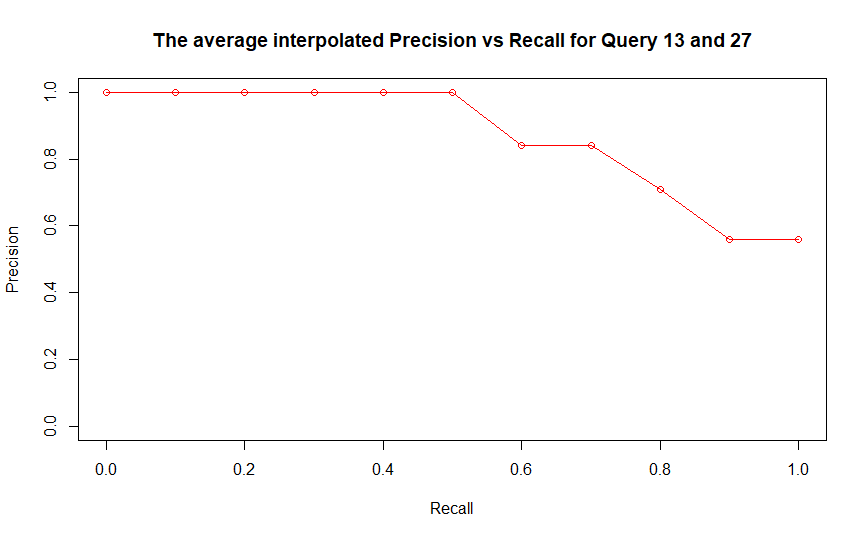
\includegraphics[scale=0.5]{Q2/a.png}
\end{figure}
